\documentclass[12pt]{jarticle}
\usepackage{TUSIReport}
\usepackage{otf}
\usepackage[dvipdfmx]{graphicx}
\usepackage[dvipdfmx]{color}
\usepackage{amsmath}
\usepackage{amssymb}
\usepackage{color}
\usepackage{hhline}
\usepackage{fancybox,ascmac}
\usepackage{multirow}
\usepackage{url}
\usepackage{bm}
\usepackage{listings,jlisting}
\lstdefinestyle{log}{
    frame={tblr},
    basicstyle={\footnotesize},
    tabsize={4},
}
\lstdefinestyle{lsthtml}{
    language={html},
    backgroundcolor={\color[gray]{.85}},
    basicstyle={\small},
    identifierstyle={\small},
    commentstyle={\small\ttfamily \color[rgb]{0,0.5,0}},
    keywordstyle={\small\bfseries \color[rgb]{1,0,0}},
    ndkeywordstyle={\small},
    stringstyle={\small\ttfamily \color[rgb]{0,0,1}},
    frame={tb},
    breaklines=true,
    columns=[l]{fullflexible},
    numbers=left,
    xrightmargin=0zw,
    xleftmargin=3zw,
    numberstyle={\scriptsize},
    stepnumber=1,
    numbersep=1zw,
    morecomment=[l]{//}
}
\lstdefinestyle{lstcpp}{
    language={C++},
    backgroundcolor={\color[gray]{.85}},
    basicstyle={\small},
    identifierstyle={\small},
    commentstyle={\small\ttfamily \color[rgb]{0,0.5,0}},
    keywordstyle={\small\bfseries \color[rgb]{1,0,0}},
    ndkeywordstyle={\small},
    stringstyle={\small\ttfamily \color[rgb]{0,0,1}},
    frame={tb},
    breaklines=true,
    columns=[l]{fullflexible},
    numbers=left,
    xrightmargin=0zw,
    xleftmargin=3zw,
    numberstyle={\scriptsize},
    stepnumber=1,
    numbersep=1zw,
    morecomment=[l]{//}
}
\begin{document}
%%%%%%%%%%%%%%%%%%%%%%%%%%%%%%%%%%%%%%%%%%%%%%%%%%%%%%%%%%%%%%
% 表紙を出力する場合は,\提出者と\共同実験者をいれる
% \提出者{科目名}{課題名}{提出年}{提出月}{提出日}{学籍番号}{氏名}
% \共同実験者{一人目}{二人目}{..}{..}{..}{..}{..}{八人目}
%%%%%%%%%%%%%%%%%%%%%%%%%%%%%%%%%%%%%%%%%%%%%%%%%%%%%%%%%%%%%%
\提出者{情報工学実験2}{実験テーマ1 数理計画法}{2020}{10}{26}{4619055}{辰川力駆}
\共同実験者{}{}{}{}{}{}{}{}

%%%%%%%%%%%%%%%%%%%%%%%%%%%%%%%%%%%%%%%%%%%%%%%%%%%%%%%%%%%%%%
% 表紙を出力しない場合は,以下の「\表紙出力」をコメントアウトする
%%%%%%%%%%%%%%%%%%%%%%%%%%%%%%%%%%%%%%%%%%%%%%%%%%%%%%%%%%%%%%
\表紙出力

%%%%%%%%%%%%%%%%%%%%%%%%%%%%%%%%%%%%%%%%%%%%%%%%%%%%%%%%%%%%%%
% 以下はレポート本体である.別途 TeXファイルを作成し \input 使っても良い
%%%%%%%%%%%%%%%%%%%%%%%%%%%%%%%%%%%%%%%%%%%%%%%%%%%%%%%%%%%%%%

\section{実験の要旨}
実験を通して、
最急降下法とニュートン法についての理解を深めるとともに、
二次元平面にプロットするなどをして議論をする。

\section{実験の目的}
非線形最適化問題に対し、
最急降下法とニュートン法を実装・適用を通し、
アルゴリズムの特性を理解する。

\section{実験の原理(理論)}
\subsection{無制約最小化問題に対する基礎理論}
無制約最小化問題とは、
$n$変数関数$f:\mathbb{R}^n \rightarrow \mathbb{R}$に対して
定義される以下の問題である。
\begin{eqnarray}
    \text{Minimize}\ f(\boldsymbol{x})\ \text{subject}\ \text{to}\ \boldsymbol{x}=(x_1,x_2,\cdots,x_n)^T \in \mathbb{R}^n\nonumber
\end{eqnarray}

\subsubsection{諸定義}
$n$変数関数$f:\mathbb{R}^n \rightarrow \mathbb{R}$に対し、
勾配ベクトル$\nabla f(\boldsymbol{x})$と
ヘッセ行列$\nabla^2f(\boldsymbol{x})$はそれぞれ以下のように
定義されるベクトルと行列である。
\begin{eqnarray}
    \nabla f(\boldsymbol{x})=\left(\begin{array}{c}
            \frac{\partial f}{\partial x_1} \\
            \vdots                          \\
            \frac{\partial f}{\partial x_n}
        \end{array}\right),\
    \nabla^2f(\boldsymbol{x})=\left(\begin{array}{ccc}
            \frac{\partial^2f}{\partial^2x_1}            & \cdots & \frac{\partial^2f}{\partial x_1\partial x_n} \\
            \vdots                                       & \ddots & \vdots                                       \\
            \frac{\partial^2f}{\partial x_n\partial x_1} & \cdots & \frac{\partial^2f}{\partial^2x_n}
        \end{array}\right)\nonumber
\end{eqnarray}
勾配ベクトルとヘッセ行列はそれぞれ1変数関数$f(\boldsymbol{x})$の
微分係数$f'(\boldsymbol{x})$と2階微分係数$f''(\boldsymbol{x})$を
$n$変数関数に拡張したものである。
ヘッセ行列は対称行列になることに注意する。
勾配ベクトルとヘッセ行列は$f$のテイラー展開に現れる。
具体的には、$\boldsymbol{x}=\boldsymbol{a}$の周りで2次の項まで求めると、
以下のようになる。
\begin{eqnarray}
    f(\boldsymbol{a}+\boldsymbol{d})=f(\boldsymbol{a})+\nabla f(\boldsymbol{a})^T\boldsymbol{d}+\frac{1}{2}\boldsymbol{d}^T\nabla^2f(\boldsymbol{a})\boldsymbol{d}+(残差)\nonumber
\end{eqnarray}
また、$n$次実正方行列$X$に対し、
\begin{itemize}
    \item $X$が半正定値とは、$X^T=X$と、$\forall\boldsymbol{d}\in\mathbb{R}^n $,\ $\boldsymbol{d}^TX\boldsymbol{d}\geq 0$が成り立つことを言い、
    \item $X$が正定値とは、$X^T=X$と、$\forall\boldsymbol{d}\in\mathbb{R}^n \backslash \{\boldsymbol{0}\}$,\ $\boldsymbol{d}^TX\boldsymbol{d}> 0$が成り立つことを言う。
\end{itemize}
さらに、$n$次実対称行列$X$に対し、
「$X$が半正定値(正定値)$\Leftrightarrow$ $X$の固有値がすべて正」が成り立つ。

\clearpage
\subsubsection{最適性条件}

一般に非線形最適化問題において大域的最適解を求めることは極めて難しく、
多くの場合は局所的最適解を求めることを目指す。
局所最適解については以下の最適性条件が成り立つ。
\begin{description}
    \item[定理](最適性の必要条件) $\boldsymbol{x}^*\in \mathbb{R}^n $を
          無制約最小化問題の局所的最適解とする。このとき、つぎが成り立つ。
          \begin{itemize}
              \item $f$が連続的微分可能$\Rightarrow \nabla f(\boldsymbol{x}^*)=\boldsymbol{0}$
              \item $f$が2回連続的微分可能$\Rightarrow \nabla^2 f(\boldsymbol{x}^*)$は半正定値行列
          \end{itemize}
          1次の必要条件$\nabla f(\boldsymbol{x}^*)=\boldsymbol{0}$を満たす
          $\boldsymbol{x}^*$を停留点という。
    \item[定理](2次の十分条件) 関数$f$が2回連続的微分可能とする。
          $\boldsymbol{x}^*\in \mathbb{R}^n$が以下の条件を満たすならば、
          $\boldsymbol{x}^*\in \mathbb{R}^n$は無制約最小化問題の局所的最適解である。
          \begin{itemize}
              \item $\nabla f(\boldsymbol{x}^*)=\boldsymbol{0}$
              \item $\nabla^2f(\boldsymbol{x}^*)$が正定値行列
          \end{itemize}
          関数が凸性と呼ばれる「良い」性質を持つ場合には、
          実は、
          大域的最適解を求めることが比較的容易になる。
          関数$f:\mathbb{R}^n \rightarrow \mathbb{R}$が
          以下の条件を満たすとき、$f$は凸関数という。
          \begin{eqnarray}
              f(\lambda\boldsymbol{x}+(1-\lambda)\boldsymbol{y})\leq \lambda f(\boldsymbol{x})+(1-\lambda)f(\boldsymbol{y}),\ \forall \boldsymbol{x},\boldsymbol{y}\in \mathbb{R}^n,\ \forall \lambda\in(0,1)\nonumber
          \end{eqnarray}
          $f$が2回連続的微分可能であるとき、以下の事実が成り立つ。
          \begin{center}
              $f$が凸関数\ $\Leftrightarrow\ \nabla^2f(\boldsymbol{x})$が半正定値行列\ \ $\forall \boldsymbol{x}\in \mathbb{R}^n$
          \end{center}
          さらに、凸関数は次の「局所最適性=大域的最適性」を満たす。
          \begin{center}
              $f$が凸関数のとき、$\boldsymbol{x}^*$が$f$の局所的最適解$\Rightarrow \boldsymbol{x}^*$は$f$の大域的最適解
          \end{center}
          これにより、微分可能な凸関数に対しては、
          $\nabla f(\boldsymbol{x}^*)=\boldsymbol{0}$を満たす
          $\boldsymbol{x}^*$を求めれば、その$\boldsymbol{x}^*$は
          最適解であることが保証される。
          このように、大域的最適解が必ず求まる関数のクラスとして、
          凸関数は重要なクラスである。
\end{description}

\clearpage
\subsection{反復法}
適当な初期点$\boldsymbol{x_0}\in \mathbb{R}^n$からスタートし、
以下の更新式で次々と点$\boldsymbol{x_1},\boldsymbol{x_2},\cdots,$を生成するアルゴリズムを反復法という。
\begin{eqnarray}
    \boldsymbol{x}_{k+1}=\boldsymbol{x}_k+\alpha_k\boldsymbol{d}_k \nonumber
\end{eqnarray}
この式における$\boldsymbol{d}_k$を探索方向、
$\alpha_k$をステップ幅という。

探索方向としては降下方向になっているものを用いるのが一般的である。
具体的には、$\boldsymbol{x} \in \mathbb{R}^n$における降下方向とは以下の条件を満たす
$\boldsymbol{d} \in \mathbb{R}^n$であり、
目的関数値が減少する方向である。
\begin{eqnarray}
    \nabla f(\boldsymbol{x})^T\boldsymbol{d} < 0 \nonumber
\end{eqnarray}
$\nabla f(\boldsymbol{x})\neq \boldsymbol{0}$であれば、
$-\nabla f(\boldsymbol{x})$
は自明な降下方向である。
これを最急降下方向という。

また、ステップ幅は次小節で説明する直線探索を利用して求めることが多い。
直線探索を用いた反復法を形式的に書くと以下のようになる。

\begin{description}
    \item[\underline{直線探索を用いた反復法}]
    \item[ステップ0:]初期点$\boldsymbol{x}_0$を選び、$k:=0$とする
    \item[ステップ1:]停止基準が満たされていれば終了とする
    \item[ステップ2:]探査方向$\boldsymbol{d}_k$を定める
    \item[ステップ3:]直線探索を用いてステップ幅$\alpha _k$を定める
    \item[ステップ4:]$\boldsymbol{x}_{k+1}:=\boldsymbol{x}_{k}+\alpha _k\boldsymbol{d}_k,\ k:=k+1$
          としてステップ幅1に戻る
\end{description}
ステップ1の停止基準としては、勾配ベクトルの大きさ
$||\nabla f(\boldsymbol{x}_k)||$が十分小さくなったことや、
解の更新幅$||\boldsymbol{x}_{k+1} - \boldsymbol{x}_k||$が
十分小さくなったことなどに設定する。

\subsection{直線探索}
点$\boldsymbol{x}_k\in \mathbb{R}^n$と$\boldsymbol{x}_k$における降下方向$\boldsymbol{d}_k$
が与えられたときに可能ならばステップ幅$\alpha _k$を
\begin{eqnarray}
    f(\boldsymbol{x}_k+\alpha_k \boldsymbol{d}_k)=\text{min}\{f(\boldsymbol{x}_k+\alpha \boldsymbol{d}_k)|\alpha > 0\}\nonumber
\end{eqnarray}
となるように選びたい。
関数$f$が凸2次関数の場合は正確に$\alpha_k$が求まるが、
そうでなければこの問題は非常に難しい(それ自体が1変数の最小化問題)。
多くの場合は次のアルミホ基準を満たすように$\alpha_k$を求める。
\clearpage
\begin{description}
    \item[定義](アルミホ基準) $0<\xi <1$を満たす定数$\xi$に対し、
          \begin{eqnarray}
              f(\boldsymbol{x}_k+\alpha\boldsymbol{d}_k) \leq f(\boldsymbol{x}_k)+\xi \alpha \nabla f(\boldsymbol{x}_k)^T \boldsymbol{d}_k \nonumber
          \end{eqnarray}
    \item[\underline{アルミホ条件に対する直線探索}]($\boldsymbol{x}_k,\boldsymbol{d}_k$は所与とする)
    \item[ステップ0:]パラメータ$0<\xi <1,0<\tau <1$を選び、$\alpha := 1$とする
    \item[ステップ1:]$f(\boldsymbol{x}_k+\alpha \boldsymbol{d}_k) \leq f(\boldsymbol{x}_k)+\xi \alpha \nabla f(\boldsymbol{x}_k)^T \boldsymbol{d}_k$(アルミホ条件)が成り立てば終了する
    \item[ステップ2:]$\alpha := \tau \alpha$としてステップ1に戻る
\end{description}
なお、アルミホ条件に$\nabla f(\boldsymbol{x}_k+\alpha \boldsymbol{d}_k)$に
関する条件を付加したウルフ条件も実用的に多く用いられている。

\subsection{実験で扱うアルゴリズム}
\subsubsection{最急降下法}
最急降下法とは、反復法におけるステップ2の探索方向として、
$\boldsymbol{x}_k$における最急降下方向$-\nabla f(\boldsymbol{x}_k)$を
常に用いる方法である。
本実験で用いる最急降下法は以下の通りである。
\begin{description}
    \item[\underline{最急降下法}]
    \item[ステップ0:] 初期点$\boldsymbol{x}_k$を選び、$k:=0$とする。
          また、$\epsilon:=10^{-8}$とする
    \item[ステップ1:] $||\nabla f(\boldsymbol{x_k})||<\epsilon$が満たされていれば終了する
    \item[ステップ2:] 探索方向を$\boldsymbol{d}_k=-\nabla f(\boldsymbol{x}_k)$とする
    \item[ステップ3:] アルミホ条件による直線探索を用いてステップ幅$\alpha_k$を定める
    \item[ステップ4:] $\boldsymbol{x}_{k+1}=\boldsymbol{x}_k+\alpha_k \boldsymbol{d}_k,\ k:=k+1$としてステップ2に戻る
\end{description}

\begin{description}
    \item[最急降下法の大域的収束性] 関数$f(\boldsymbol{x})$に関するいくつかの仮定の下では
          ウルフ条件を用いた最急降下法は任意の初期点に対して以下の式が成り立つ。
          \begin{eqnarray}
              \lim_{k\rightarrow \infty}||\nabla f(\boldsymbol{x}_k)||=0\nonumber
          \end{eqnarray}
          このように、初期点に依存せずに停留点に収束するのは
          最急降下法の強みであるが、その一方で収束スピードが非常に遅い欠点を持つ。
    \item[最急降下法の1次収束性] 最急降下法で生成される点列$\{\boldsymbol{x}_k\}$の収束先を$\boldsymbol{x}^*$とすると
          以下の式が成り立つ定数$0<c<1$が存在する。
          \begin{eqnarray}
              ||\boldsymbol{x}_{k+1}-\boldsymbol{x}^*||\leq c||\boldsymbol{x}_{k}-\boldsymbol{x}^*||\nonumber
          \end{eqnarray}
          この式では一見、
          収束が遅いようには見えないが、$\boldsymbol{x}^*$付近では$||\boldsymbol{x}_{k}-\boldsymbol{x}^*||$が
          非常に微小のため、最急降下法が収束するまでに要する反復数は非常に多い。
\end{description}

\subsubsection{ニュートン法}
ニュートン法は$f(\boldsymbol{x})$2次の項までのテイラー展開を
最小化することを繰り返す方法である。すなわち、

\begin{eqnarray}
    q(\boldsymbol{d})=f(\boldsymbol{x}_k+\boldsymbol{d})=f(\boldsymbol{x}_k)+\nabla f(\boldsymbol{x}_k)^T \boldsymbol{d}+\frac{1}{2}\boldsymbol{d}^T \nabla^2 f(\boldsymbol{x}_k)\boldsymbol{d}\nonumber
\end{eqnarray}
として、$\nabla q(\boldsymbol{d})=\nabla f(\boldsymbol{x}_k)+\nabla^2 f(\boldsymbol{x}_k)\boldsymbol{d}=\boldsymbol{0}$を満たす
$\boldsymbol{d}$を探索方向とする。
方向$\boldsymbol{d}$はニュートン方向と呼ばれ、
以下のニュートン方程式を解くことで得られる。

\begin{eqnarray}
    \nabla^2f(\boldsymbol{x}_k)\boldsymbol{d}=-\nabla f(\boldsymbol{x}_k)\nonumber
\end{eqnarray}
本実験で用いるニュートン法は以下の通りである。

\begin{description}
    \item [\underline{ニュートン法}]
    \item [ステップ0:] 初期点$\boldsymbol{x}_0$を選び、$k=0$とする。
          $\epsilon=10^{-8}$とする
    \item [ステップ1:] $||\nabla f(\boldsymbol{x_k})||<\epsilon$が
          満たされていれば終了する
    \item [ステップ2:] 方程式$\nabla^2 f(\boldsymbol{x}_k)\boldsymbol{d}=-\nabla f(\boldsymbol{x}_k)$を解いて探索方向$\boldsymbol{d}_k$を求める
    \item [ステップ3:] $\boldsymbol{x}_{k+1}:=\boldsymbol{x}_k+\boldsymbol{d}_k,\ k:=k+1$としてステップ1に戻る
\end{description}

\begin{description}
    \item[ニュートン法の局所的2次収束性] 初期点$\boldsymbol{x}_0$を$\boldsymbol{x}^*$の
          十分近くに点を取ると、ニュートン法で生成される点列$\{\boldsymbol{x}_k\}$は収束し、
          その収束先を$\boldsymbol{x}^*$とすると以下を満たす定数$c\geq 0$が存在する。
          \begin{eqnarray}
              ||\boldsymbol{x}_{k+1}-\boldsymbol{x}^*||\leq c||\boldsymbol{x}_{k}-\boldsymbol{x}^*||^2\nonumber
          \end{eqnarray}
          1次収束と異なり、
          上の2次収束は非常に速い。
          一方で、初期点の取り方が悪ければニュートン法は収束しなかったり、
          局所最適解でない点に収束することもしばしばある。
\end{description}

\clearpage

\section{実験課題}
次の各項目に取り組む。
\begin{itemize}
    \item [(1)]実験目的とアルゴリズムに関する数学的理論について概要を述べる。
    \item [(2)]以下の2種類の2変数関数に対して最急降下法を実行するプログラムを完成させる。
          \begin{eqnarray}
              f_1(x_1,x_2)&=&\frac{1}{2}
              \left(\begin{array}{c}
                      x_1 \\
                      x_2
                  \end{array}\right)^T\left(\begin{array}{cc}
                      p & q \\
                      q & r
                  \end{array}\right)\left(\begin{array}{c}
                      x_1 \\
                      x_2
                  \end{array}\right)+\left(\begin{array}{c}
                      c_1 \\
                      c_2
                  \end{array}\right)^T\left(\begin{array}{c}
                      x_1 \\
                      x_2
                  \end{array}\right)+e^{(x_1-x_2)^2}\nonumber\\
              f_2(x_1,x_2)&=&\sum^4_{i=0}\sum^2_{j=0}a_{ij}x^i_1x^j_2\nonumber
          \end{eqnarray}
    \item [(3)](2)で作成したプログラムを動かしてふるまいを観察し、性能を考察する。
    \item [(4)]関数$f_1$と関数$f_2$に対してニュートン法
          を実行するプログラムを完成させる。
    \item [(5)](4)で作成したプログラムを動かしてふるまいを観察し、性能を考察する。
\end{itemize}

\section{実験結果・検討・考察}
\subsection*{(1)}
上記(目的、原理)で述べた。
\subsection*{(2)}
それぞれの関数に対して作成したソースコード2つを付録に載せた。
$f_1$のソースコードも$f_2$のソースコードも仕組みは同じなのでソースコード1(4619055\_辰川力駆\_SD\_1.c)
に対しての説明をする。

まず、27行目から48行目でファイルを読み取り、最急降下法を使う行列を受け取っている。
そして、確認のために50行目から71行目で出力している。
次に、メインの最急降下法(77行目から114行目)について説明する。
79行目から83行目までは$\nabla f(\boldsymbol{x}_k)$と$\boldsymbol{d}_k$を求めている。
その後、ノルム、関数値を求めた後に、アルミホ条件による直線探索を用いてステップ幅を定めている。
アルミホ条件によるステップ幅の決定は116行目から142行目の関数で求めている。

最後に$\boldsymbol{x}_k$を更新したあと、101行目から108行目で終了条件が満たされていれば終了する。
満たされていなければさらに実行というようにしている。
$||\nabla f(\boldsymbol{x_k})||<\epsilon$という条件だけでは、
最急降下法はたくさんの回数を要するため時間がかかってしまう可能性があるので
反復回数が1000回を越えたら停止するように工夫している。

出力部分に関しては、反復回数、現在位置、目的関数、勾配ベクトル、ノルムを表示するようにした。
表示する頻度は多すぎるといけないので、0,1,2,3,4,5,10,20,30,40,50,60,70,80,90,100,200,300,
400,500,600,700,800,900,1000
とするように工夫をした。

\subsection*{(3)}

学籍番号は4619055なのでseed値を55としてデータを発生させた。
実験に用いるデータは下記である。なお、図2の一番右のデータはdata55.txtのデータである。
\begin{figure}[h]
    \begin{minipage}{0.3\hsize}
        \begin{center}
            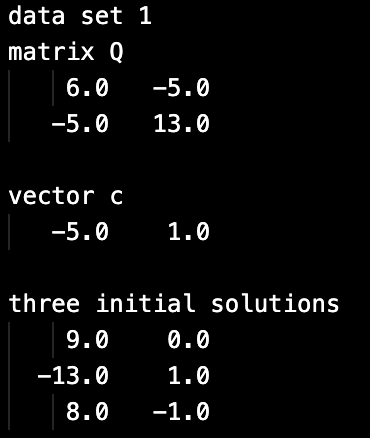
\includegraphics[scale=0.35]{kadai1_1data1.png}
        \end{center}
    \end{minipage}
    \begin{minipage}{0.3\hsize}
        \begin{center}
            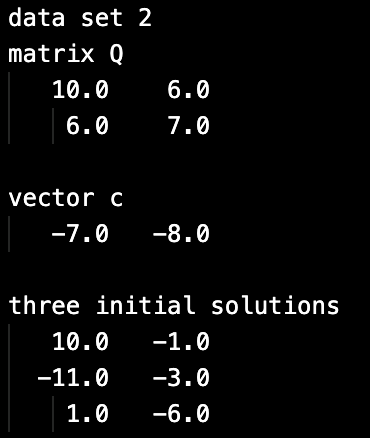
\includegraphics[scale=0.35]{kadai1_1data2.png}
        \end{center}
    \end{minipage}
    \begin{minipage}{0.3\hsize}
        \begin{center}
            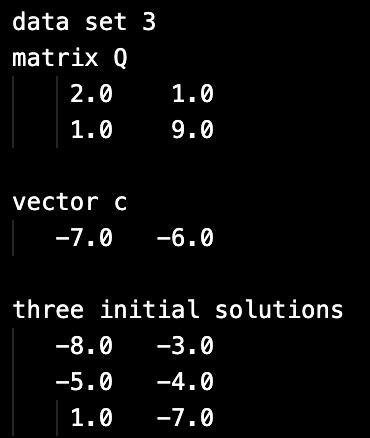
\includegraphics[scale=0.35]{kadai1_1data3.png}
        \end{center}
    \end{minipage}
    \caption{$f_1$で用いる実験データ}
\end{figure}

\begin{figure}[h]
    \begin{minipage}{0.3\hsize}
        \begin{center}
            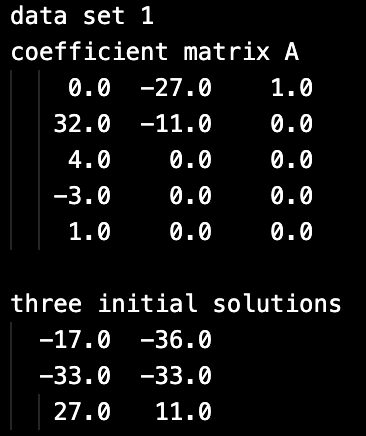
\includegraphics[scale=0.35]{kadai1_2data1.png}
        \end{center}
    \end{minipage}
    \begin{minipage}{0.3\hsize}
        \begin{center}
            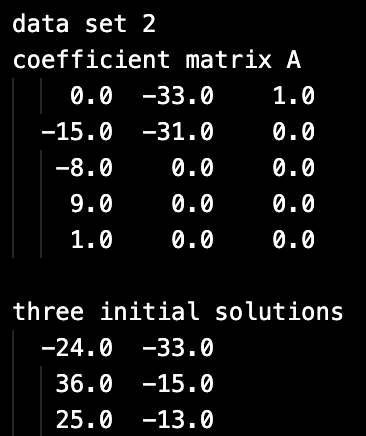
\includegraphics[scale=0.35]{kadai1_2data2.png}
        \end{center}
    \end{minipage}
    \begin{minipage}{0.3\hsize}
        \begin{center}
            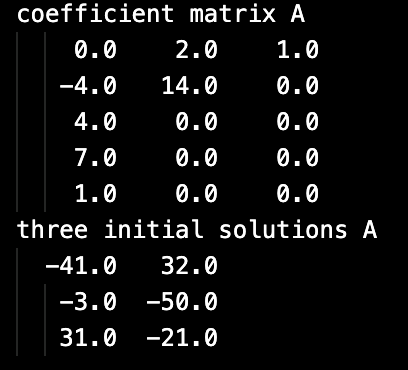
\includegraphics[scale=0.4]{kadai1_2data3.png}
        \end{center}
    \end{minipage}
    \caption{$f_2$で用いる実験データ}
\end{figure}

実行結果は以下のようになった。
\begin{figure}[h]
    \begin{minipage}{0.3\hsize}
        \begin{center}
            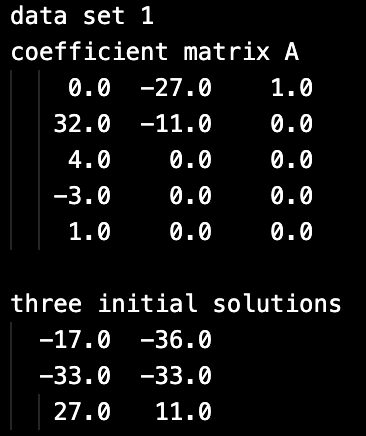
\includegraphics[scale=0.35]{kadai1_2data1.png}
        \end{center}
    \end{minipage}
    \begin{minipage}{0.3\hsize}
        \begin{center}
            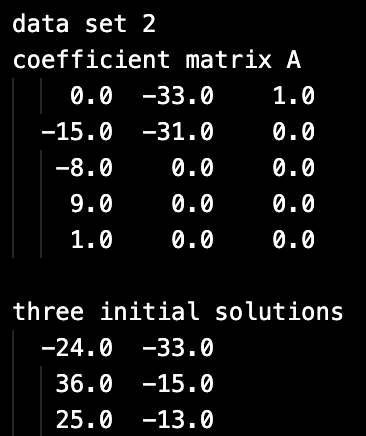
\includegraphics[scale=0.35]{kadai1_2data2.png}
        \end{center}
    \end{minipage}
    \begin{minipage}{0.3\hsize}
        \begin{center}
            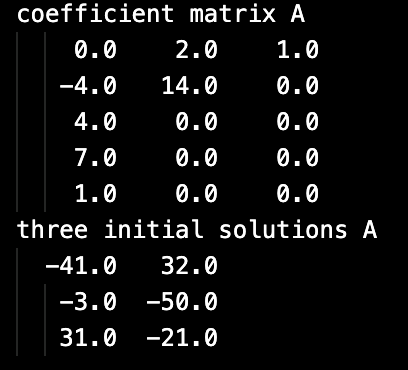
\includegraphics[scale=0.4]{kadai1_2data3.png}
        \end{center}
    \end{minipage}
    \caption{$f_1$,\ data set 1,\ $\boldsymbol{x}_0$の値1行目の結果}
\end{figure}
\begin{figure}[h]
    \begin{minipage}{0.3\hsize}
        \begin{center}
            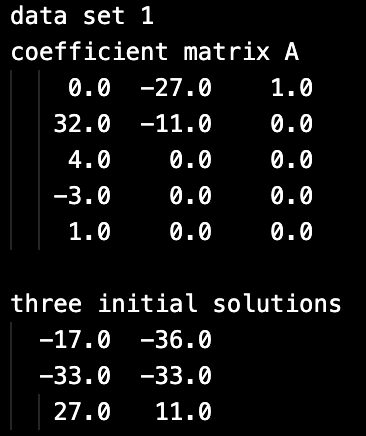
\includegraphics[scale=0.35]{kadai1_2data1.png}
        \end{center}
    \end{minipage}
    \begin{minipage}{0.3\hsize}
        \begin{center}
            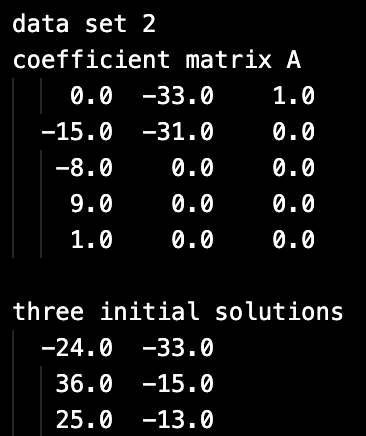
\includegraphics[scale=0.35]{kadai1_2data2.png}
        \end{center}
    \end{minipage}
    \begin{minipage}{0.3\hsize}
        \begin{center}
            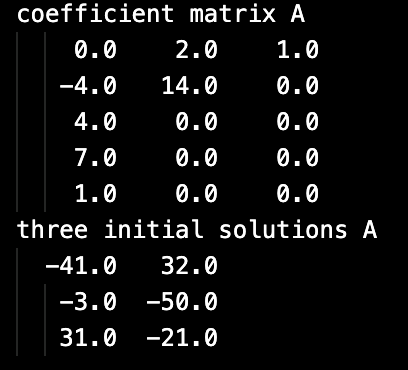
\includegraphics[scale=0.4]{kadai1_2data3.png}
        \end{center}
    \end{minipage}
    \caption{$f_1$,\ data set 1,\ $\boldsymbol{x}_0$の値2行目の結果}
\end{figure}
\begin{figure}[h]
    \begin{minipage}{0.3\hsize}
        \begin{center}
            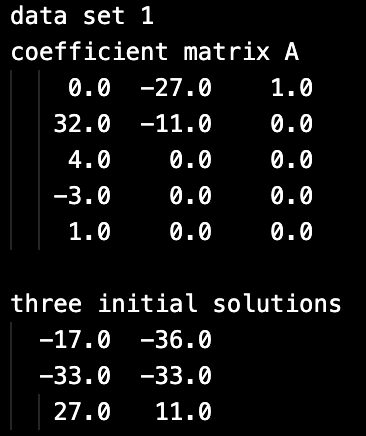
\includegraphics[scale=0.35]{kadai1_2data1.png}
        \end{center}
    \end{minipage}
    \begin{minipage}{0.3\hsize}
        \begin{center}
            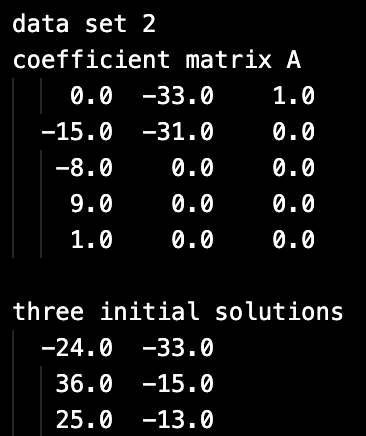
\includegraphics[scale=0.35]{kadai1_2data2.png}
        \end{center}
    \end{minipage}
    \begin{minipage}{0.3\hsize}
        \begin{center}
            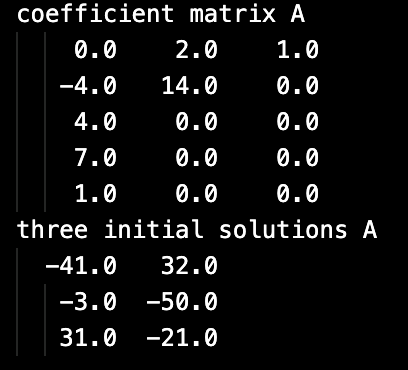
\includegraphics[scale=0.4]{kadai1_2data3.png}
        \end{center}
    \end{minipage}
    \caption{$f_1$,\ data set 1,\ $\boldsymbol{x}_0$の値3行目の結果}
\end{figure}

\clearpage
\subsection*{(4)}
それぞれの関数に対して作成したソースコード2つを付録に載せた。
$f_1$のソースコードも$f_2$のソースコードも仕組みは同じなのでソースコード3(4619055\_辰川力駆\_newton\_1.c)
に対しての説明をする。

まず、29行目から50行目でファイルを読み取り、ニュートン法を使う行列を受け取っている。
そして、確認のために52行目から73行目で出力している。
次に、メインの最急降下法(79行目から111行目)について説明する。
81,82行目では$\nabla f(\boldsymbol{x}_k)$を求めている。
その後、ノルム、探索方向$\boldsymbol{d}_k$、関数値を求めている。
探索方向はニュートン法を使っている。ニュートン法は関数化している。
ニュートン法では、まずヘッセ行列$\nabla^2 f(\boldsymbol{x_k})$を求めて、
正則でなければ、$\boldsymbol{d}=\text{inf}$としている。
正則であればヘッセ行列の逆行列を求めて、$\boldsymbol{d}$を計算している。

最後に$\boldsymbol{x}_k$を更新したあと、98行目から110行目で終了条件が満たされていれば終了する。
満たされていなければさらに実行というようにしている。
$||\nabla f(\boldsymbol{x_k})||<\epsilon$という停止条件と
反復回数が500回を超えるという停止条件以外に
$\nabla^2 f(\boldsymbol{x_k})$が非正則なら停止するようにしている。

出力部分に関しては最急降下法と同様に、反復回数、現在位置、目的関数、勾配ベクトル、ノルムを表示するようにした。
表示する頻度は多すぎるといけないので、0,1,2,3,4,5,10,20,30,40,50,60,70,
80,90,100,200,300,400,500,600,700,800,900,1000
とするように工夫をした。

\subsection*{(5)}
ニュートン法は非正則になったら終了しないといけないのでつらい

\section{まとめ}
最急降下法とニュートン法をC言語で実装した。
また、それらの適用を通し、
アルゴリズムの特性を理解することができた。

\clearpage

% 参考文献
\begin{thebibliography}{99}
    \label{sannkoubunnkenn_chapter}
    \bibitem[1]{rikadai}東京理科大学工学部情報工学科 情報工学実験2 2020年度
    東京理科大学工学部情報工学科出版

    \bibitem[2]{toukei}
    関数グラフ - GeoGebra

    \url{https://www.geogebra.org/graphing?lang=ja}

    最終閲覧日2020/10/29

\end{thebibliography}


\clearpage

% 付録
\appendix
\section{付録}
\begin{lstlisting}[style = lstcpp,caption=4619055\_辰川力駆\_SD\_1.c]
    //4619055 辰川力駆
    #include <stdio.h>
    #include <stdlib.h>
    #include <string.h>
    #include <math.h>
    #define N 1000
    #define res 0.00000001 ///停止条件
    
    double func(double *x);                             ///f1の式を用いている
    double Armijo(double *x, double *d, double *nabla); //Armijo
    
    double Q[2][2]; //Qのデータを保存
    double c[2];    //cのデータを保存
    
    int main()
    {
        char fname[128];
        double x[2];
        double p, q, r;
        double d[2], norm;
        double nabla[2];
        double f;
        FILE *fp;
        int i, j, k;
        double alpha;
    
        printf("input filename:");
        fgets(fname, sizeof(fname), stdin);
        fname[strlen(fname) - 1] = '\0';
        fflush(stdin);
        fp = fopen(fname, "r");
    
        for (i = 0; i < 2; i++)
        {
            for (j = 0; j < 2; j++)
            {
                fscanf(fp, "%lf", &Q[i][j]);
            }
        }
        for (i = 0; i < 2; i++)
        {
            fscanf(fp, "%lf", &c[i]);
        }
        for (i = 0; i < 2; i++)
        {
            fscanf(fp, "%lf", &x[i]);
        }
        fclose(fp);
    
        printf("Q=\n");
        for (i = 0; i < 2; i++)
        {
            for (j = 0; j < 2; j++)
            {
                printf("%4.lf", Q[i][j]);
            }
            printf("\n");
        }
        printf("C=\n");
        for (i = 0; i < 2; i++)
        {
            printf("%4.lf", c[i]);
        }
        printf("\n");
        printf("x=\n");
        for (i = 0; i < 2; i++)
        {
            printf("%4.lf", x[i]);
        }
        printf("\n");
        printf("-----\n");
    
        p = Q[0][0];
        q = Q[0][1];
        r = Q[1][1];
        k = 0;
        while (1)
        {
            nabla[0] = p * x[0] + q * x[1] + c[0] + 2 * (x[0] - x[1]) * exp((x[0] - x[1]) * (x[0] - x[1]));
            nabla[1] = q * x[0] + r * x[1] + c[1] - 2 * (x[0] - x[1]) * exp((x[0] - x[1]) * (x[0] - x[1]));
    
            d[0] = -nabla[0];
            d[1] = -nabla[1];
    
            norm = sqrt(nabla[0] * nabla[0] + nabla[1] * nabla[1]); ///ノルムを計算
    
            f = func(x);
            alpha = Armijo(x, d, nabla);
    
            if (k <= 5 || (k <= 100 && k % 10 == 0) || k % 100 == 0) //5回目までと10n回目,100n回目(n=1,2,3,...10)を表示
            {
                printf("%d回目\n", k);
                printf("現在位置=(%.8lf,%.8lf)\n目的関数=%.8lf\n勾配ベクトル=(%.8lf,%.8lf)\nノルム=%.8lf\n", x[0], x[1], f, nabla[0], nabla[1], norm);
                printf("-----\n");
            }
    
            x[0] = x[0] + alpha * d[0];
            x[1] = x[1] + alpha * d[1];
            k++;
    
            if (norm < res) ///nablaのノルムが10^{-8}を越えていたら停止
            {
                break;
            }
            if (k > N) ///反復回数が1000回越えたら停止
            {
                break;
            }
        }
    
        printf("--結果--\n");
        printf("%d回\n現在位置=(%.8lf,%.8lf)\n目的関数=%.8lf\n勾配ベクトル=(%.8lf,%.8lf)\nノルム=%.8lf\n", k - 1, x[0], x[1], f, nabla[0], nabla[1], norm);
        return 0;
    }
    
    double Armijo(double *x, double *d, double *nabla)
    {
        double alpha = 1.0;
        double xi = 0.1;  ///今回の課題条件
        double tau = 0.5; ///今回の課題条件
        double fx, fy;
        double y[2];
    
        ///f(x_k)を求める
        fx = func(x);
    
        while (1)
        {
            ///新しいalphaに対してのfyを求める
            y[0] = x[0] + alpha * d[0];
            y[1] = x[1] + alpha * d[1];
            fy = func(y);
    
            if (fy <= fx + xi * (nabla[0] * d[0] + nabla[1] * d[1]) * alpha) //Armijo条件
            {
                break;
            }
    
            alpha = tau * alpha; //alphaの更新
        }
        return alpha;
    }
    
    // f1の式を用いている
    double func(double *x)
    {
        double p, q, r;
        p = Q[0][0];
        q = Q[0][1];
        r = Q[1][1];
        return 0.5 * (p * x[0] * x[0] + 2 * q * x[0] * x[1] + r * x[1] * x[1]) + c[0] * x[0] + c[1] * x[1] + exp((x[0] - x[1]) * (x[0] - x[1]));
    }
\end{lstlisting}

\begin{lstlisting}[style = lstcpp,caption=4619055\_辰川力駆\_SD\_2.c]
    //4619055 辰川力駆
    #include <stdio.h>
    #include <stdlib.h>
    #include <string.h>
    #include <math.h>
    #define N 1000
    #define res 0.00000001 ///停止条件
    
    double func(double *x);                             ///f2の式を用いている
    double Armijo(double *x, double *d, double *nabla); //Armijo
    
    double A[5][3]; //Aのデータを保存
    
    int main()
    {
        char fname[128];
        double x[2];
        double d[2], norm;
        double nabla[2];
        double f;
        FILE *fp;
        int i, j, k;
        double alpha;
    
        printf("input filename:");
        fgets(fname, sizeof(fname), stdin);
        fname[strlen(fname) - 1] = '\0';
        fflush(stdin);
        fp = fopen(fname, "r");
    
        for (i = 0; i < 5; i++)
        {
            for (j = 0; j < 3; j++)
            {
                fscanf(fp, "%lf", &A[i][j]);
            }
        }
        for (i = 0; i < 2; i++)
        {
            fscanf(fp, "%lf", &x[i]);
        }
        fclose(fp);
    
        printf("A=\n");
        for (i = 0; i < 5; i++)
        {
            for (j = 0; j < 3; j++)
            {
                printf("%4.lf", A[i][j]);
            }
            printf("\n");
        }
        printf("x=\n");
        for (i = 0; i < 2; i++)
        {
            printf("%4.lf", x[i]);
        }
        printf("\n");
        printf("-----\n");
    
        k = 0;
        while (1)
        {
            nabla[0] = A[1][0] + A[1][1] * x[1] + 2 * A[2][0] * x[0] + 3 * A[3][0] * pow(x[0], 2) + 4 * A[4][0] * pow(x[0], 3);
            nabla[1] = A[0][1] + 2 * A[0][2] * x[1] + A[1][1] * x[0];
    
            d[0] = -nabla[0];
            d[1] = -nabla[1];
    
            norm = sqrt(nabla[0] * nabla[0] + nabla[1] * nabla[1]); ///ノルムを計算
    
            f = func(x);
            alpha = Armijo(x, d, nabla);
    
            if (k <= 5 || (k <= 100 && k % 10 == 0) || k % 100 == 0) //5回目までと10n回目,100n回目(n=1,2,3,...10)を表示
            {
                printf("%d回目\n", k);
                printf("現在位置=(%.8lf,%.8lf)\n目的関数=%.8lf\n勾配ベクトル=(%.8lf,%.8lf)\nノルム=%.8lf\n", x[0], x[1], f, nabla[0], nabla[1], norm);
                printf("-----\n");
            }
    
            x[0] = x[0] + alpha * d[0];
            x[1] = x[1] + alpha * d[1];
            k++;
    
            if (norm < res) ///nablaのノルムが10^{-8}を越えていたら停止
            {
                break;
            }
            if (k > N) ///反復回数が1000回越えたら停止
            {
                break;
            }
        }
    
        printf("--結果--\n");
        printf("%d回\n現在位置=(%.8lf,%.8lf)\n目的関数=%.8lf\n勾配ベクトル=(%.8lf,%.8lf)\nノルム=%.8lf\n", k - 1, x[0], x[1], f, nabla[0], nabla[1], norm);
        return 0;
    }
    
    double Armijo(double *x, double *d, double *nabla)
    {
        double alpha = 1.0;
        double xi = 0.1;  ///今回の課題条件
        double tau = 0.5; ///今回の課題条件
        double fx, fy;
        double y[2];
    
        ///f(x_k)を求める
        fx = func(x);
    
        while (1)
        {
            ///新しいalphaに対してのfyを求める
            y[0] = x[0] + alpha * d[0];
            y[1] = x[1] + alpha * d[1];
            fy = func(y);
    
            if (fy <= fx + xi * (nabla[0] * d[0] + nabla[1] * d[1]) * alpha) //Armijo条件
            {
                break;
            }
    
            alpha = tau * alpha; //alphaの更新
        }
        return alpha;
    }
    
    //f2の式を用いている
    double func(double *x)
    {
        return A[0][1] * x[1] + A[0][2] * pow(x[1], 2) + A[1][0] * x[0] + A[1][1] * x[0] * x[1] + A[2][0] * pow(x[0], 2) + A[3][0] * pow(x[0], 3) + A[4][0] * pow(x[0], 4);
    }
\end{lstlisting}

\begin{lstlisting}[style = lstcpp,caption=4619055\_辰川力駆\_newton\_1.c]
    //4619055 辰川力駆
    #include <stdio.h>
    #include <stdlib.h>
    #include <string.h>
    #include <math.h>
    #define inf 10000000000000
    #define N 500
    #define res 0.00000001 ///停止条件
    
    double func(double *x);                           ///f1の式を用いている
    void Hf(double *x, double *d);                    ///ヘッセ行列を求める
    void Newton(double *x, double *d, double *nabla); //dを計算する
    
    double Q[2][2];       //Qのデータを保存
    double c[2];          //cのデータを保存
    double Hessian[2][2]; ///ヘッセ行列を保存
    
    int main()
    {
        char fname[128];
        double x[2];
        double p, q, r;
        double d[2], norm;
        double nabla[2];
        double f;
        FILE *fp;
        int i, j, k;
    
        printf("input filename:");
        fgets(fname, sizeof(fname), stdin);
        fname[strlen(fname) - 1] = '\0';
        fflush(stdin);
        fp = fopen(fname, "r");
    
        for (i = 0; i < 2; i++)
        {
            for (j = 0; j < 2; j++)
            {
                fscanf(fp, "%lf", &Q[i][j]);
            }
        }
        for (i = 0; i < 2; i++)
        {
            fscanf(fp, "%lf", &c[i]);
        }
        for (i = 0; i < 2; i++)
        {
            fscanf(fp, "%lf", &x[i]);
        }
        fclose(fp);
    
        printf("Q=\n");
        for (i = 0; i < 2; i++)
        {
            for (j = 0; j < 2; j++)
            {
                printf("%4.lf", Q[i][j]);
            }
            printf("\n");
        }
        printf("C=\n");
        for (i = 0; i < 2; i++)
        {
            printf("%4.lf", c[i]);
        }
        printf("\n");
        printf("x=\n");
        for (i = 0; i < 2; i++)
        {
            printf("%4.lf", x[i]);
        }
        printf("\n");
        printf("-----\n");
    
        p = Q[0][0];
        q = Q[0][1];
        r = Q[1][1];
        k = 0;
        while (1)
        {
            nabla[0] = p * x[0] + q * x[1] + c[0] + 2 * (x[0] - x[1]) * exp((x[0] - x[1]) * (x[0] - x[1]));
            nabla[1] = q * x[0] + r * x[1] + c[1] - 2 * (x[0] - x[1]) * exp((x[0] - x[1]) * (x[0] - x[1]));
    
            norm = sqrt(nabla[0] * nabla[0] + nabla[1] * nabla[1]); ///ノルムを計算
    
            Newton(x, d, nabla); //dを計算
            f = func(x);
    
            if (k <= 5 || (k <= 100 && k % 10 == 0) || k % 100 == 0) //5回目までと10n回目,100n回目(n=1,2,3,...10)を表示
            {
                printf("%d回目\n", k);
                printf("現在位置=(%.8lf,%.8lf)\n目的関数=%.8lf\n勾配ベクトル=(%.8lf,%.8lf)\nノルム=%.8lf\n", x[0], x[1], f, nabla[0], nabla[1], norm);
                printf("-----\n");
            }
            x[0] = x[0] + d[0];
            x[1] = x[1] + d[1];
            k++;
            if (norm < res) ///nablaのノルムが10^{-8}を越えていたら停止
            {
                break;
            }
            if (k > N) ///反復回数が500回越えたら停止
            {
                break;
            }
            if (d[0] == inf) ///nabla^2が非正則なら停止
            {
                printf("非正則なので終了します\n");
                break;
            }
        }
        printf("--結果--\n");
        printf("%d回\n現在位置=(%.8lf,%.8lf)\n目的関数=%.8lf\n勾配ベクトル=(%.8lf,%.8lf)\nノルム=%.8lf\n", k - 1, x[0], x[1], f, nabla[0], nabla[1], norm);
        return 0;
    }
    
    void Newton(double *x, double *d, double *nabla)
    {
        double Hessian_inverse[2][2];
        Hf(x, d);
        if (Hessian[0][0] * Hessian[1][1] - Hessian[0][1] * Hessian[1][0] == 0) ///正則かどうか
        {
            d[0] = inf;
            d[1] = inf;
        }
        else
        {
            Hessian_inverse[0][0] = 1 / (Hessian[0][0] * Hessian[1][1] - Hessian[0][1] * Hessian[1][0]) * Hessian[1][1];
            Hessian_inverse[0][1] = 1 / (Hessian[0][0] * Hessian[1][1] - Hessian[0][1] * Hessian[1][0]) * -Hessian[0][1];
            Hessian_inverse[1][0] = 1 / (Hessian[0][0] * Hessian[1][1] - Hessian[0][1] * Hessian[1][0]) * -Hessian[1][0];
            Hessian_inverse[1][1] = 1 / (Hessian[0][0] * Hessian[1][1] - Hessian[0][1] * Hessian[1][0]) * Hessian[0][0];
            d[0] = -(Hessian_inverse[0][0] * nabla[0] + Hessian_inverse[1][0] * nabla[1]);
            d[1] = -(Hessian_inverse[0][1] * nabla[0] + Hessian_inverse[1][1] * nabla[1]);
        }
    }
    
    void Hf(double *x, double *d)
    {
        double p, q, r;
        p = Q[0][0];
        q = Q[0][1];
        r = Q[1][1];
        Hessian[0][0] = p + 2 * (1 + 2 * pow(x[0] - x[1], 2)) * exp(pow(x[0] - x[1], 2));
        Hessian[0][1] = q - 2 * (1 + 2 * pow(x[0] - x[1], 2)) * exp(pow(x[0] - x[1], 2));
        Hessian[1][0] = Hessian[0][1];
        Hessian[1][1] = r + 2 * (1 + 2 * pow(x[0] - x[1], 2)) * exp(pow(x[0] - x[1], 2));
    }
    
    // f1の式を用いている
    double func(double *x)
    {
        double p, q, r;
        p = Q[0][0];
        q = Q[0][1];
        r = Q[1][1];
        return 0.5 * (p * x[0] * x[0] + 2 * q * x[0] * x[1] + r * x[1] * x[1]) + c[0] * x[0] + c[1] * x[1] + exp((x[0] - x[1]) * (x[0] - x[1]));
    }
\end{lstlisting}

\begin{lstlisting}[style = lstcpp,caption=4619055\_辰川力駆\_newton\_2.c]
    //4619055 辰川力駆
    #include <stdio.h>
    #include <stdlib.h>
    #include <string.h>
    #include <math.h>
    #define inf 10000000000000
    #define N 500
    #define res 0.00000001 ///停止条件
    
    double func(double *x);                           ///f2の式を用いている
    void Hf(double *x, double *d);                    ///ヘッセ行列を求める
    void Newton(double *x, double *d, double *nabla); //dを計算する
    
    double A[5][3];       //Aのデータを保存
    double Hessian[2][2]; ///ヘッセ行列を保存
    
    int main()
    {
        char fname[128];
        double x[2];
        double d[2], norm;
        double nabla[2];
        double f;
        FILE *fp;
        int i, j, k;
    
        printf("input filename:");
        fgets(fname, sizeof(fname), stdin);
        fname[strlen(fname) - 1] = '\0';
        fflush(stdin);
        fp = fopen(fname, "r");
    
        for (i = 0; i < 5; i++)
        {
            for (j = 0; j < 3; j++)
            {
                fscanf(fp, "%lf", &A[i][j]);
            }
        }
        for (i = 0; i < 2; i++)
        {
            fscanf(fp, "%lf", &x[i]);
        }
        fclose(fp);
    
        printf("A=\n");
        for (i = 0; i < 5; i++)
        {
            for (j = 0; j < 3; j++)
            {
                printf("%4.lf", A[i][j]);
            }
            printf("\n");
        }
        printf("x=\n");
        for (i = 0; i < 2; i++)
        {
            printf("%4.lf", x[i]);
        }
        printf("\n");
        printf("-----\n");
    
        k = 0;
        while (1)
        {
            nabla[0] = A[1][0] + A[1][1] * x[1] + 2 * A[2][0] * x[0] + 3 * A[3][0] * pow(x[0], 2) + 4 * A[4][0] * pow(x[0], 3);
            nabla[1] = A[0][1] + 2 * A[0][2] * x[1] + A[1][1] * x[0];
    
            norm = sqrt(nabla[0] * nabla[0] + nabla[1] * nabla[1]); ///ノルムを計算
    
            Newton(x, d, nabla); //dを計算
            f = func(x);
            if (k <= 5 || (k <= 100 && k % 10 == 0) || k % 100 == 0) //5回目までと10n回目,100n回目(n=1,2,3,...10)を表示
            {
                printf("%d回目\n", k);
                printf("現在位置=(%.8lf,%.8lf)\n目的関数=%.8lf\n勾配ベクトル=(%.8lf,%.8lf)\nノルム=%.8lf\n", x[0], x[1], f, nabla[0], nabla[1], norm);
                printf("-----\n");
            }
            x[0] = x[0] + d[0];
            x[1] = x[1] + d[1];
            k++;
            if (norm < res) ///nablaのノルムが10^{-8}を越えていたら停止
            {
                break;
            }
            if (k > N) ///反復回数が500回越えたら停止
            {
                break;
            }
            if (d[0] == inf) ///nabla^2が非正則なら停止
            {
                printf("非正則なので終了します\n");
                break;
            }
        }
    
        printf("--結果--\n");
        printf("%d回\n現在位置=(%.8lf,%.8lf)\n目的関数=%.8lf\n勾配ベクトル=(%.8lf,%.8lf)\nノルム=%.8lf\n", k - 1, x[0], x[1], f, nabla[0], nabla[1], norm);
        return 0;
    }
    
    void Newton(double *x, double *d, double *nabla)
    {
        double Hessian_inverse[2][2];
        Hf(x, d);
        if (Hessian[0][0] * Hessian[1][1] - Hessian[0][1] * Hessian[1][0] == 0) ///正則かどうか
        {
            d[0] = inf;
            d[1] = inf;
        }
        else
        {
            Hessian_inverse[0][0] = 1 / (Hessian[0][0] * Hessian[1][1] - Hessian[0][1] * Hessian[1][0]) * Hessian[1][1];
            Hessian_inverse[0][1] = 1 / (Hessian[0][0] * Hessian[1][1] - Hessian[0][1] * Hessian[1][0]) * -Hessian[0][1];
            Hessian_inverse[1][0] = 1 / (Hessian[0][0] * Hessian[1][1] - Hessian[0][1] * Hessian[1][0]) * -Hessian[1][0];
            Hessian_inverse[1][1] = 1 / (Hessian[0][0] * Hessian[1][1] - Hessian[0][1] * Hessian[1][0]) * Hessian[0][0];
            d[0] = -(Hessian_inverse[0][0] * nabla[0] + Hessian_inverse[1][0] * nabla[1]);
            d[1] = -(Hessian_inverse[0][1] * nabla[0] + Hessian_inverse[1][1] * nabla[1]);
        }
    }
    
    void Hf(double *x, double *d)
    {
        Hessian[0][0] = 2 * A[2][0] + 6 * A[3][0] * x[0] + 12 * A[4][0] * pow(x[0], 2);
        Hessian[0][1] = A[1][1];
        Hessian[1][0] = Hessian[0][1];
        Hessian[1][1] = 2 * A[0][2];
    }
    
    //f2の式を用いている
    double func(double *x)
    {
        return A[0][1] * x[1] + A[0][2] * pow(x[1], 2) + A[1][0] * x[0] + A[1][1] * x[0] * x[1] + A[2][0] * pow(x[0], 2) + A[3][0] * pow(x[0], 3) + A[4][0] * pow(x[0], 4);
    }
\end{lstlisting}

%%%%%%%%%%%%%%%%%%%%%%%%%%%%%%%%%%%%%%%%%%%%%%%%%%%%%%%%%%%%%%
\end{document}